\documentclass[11pt,a4paper]{report}
\usepackage[margin=1in]{geometry}
\usepackage{amsmath, amsfonts, amssymb, amsthm}
% Use only algorithm2e for algorithms, not algorithm/algorithmic
\usepackage[ruled,vlined,linesnumbered]{algorithm2e}
\usepackage{listings}
\usepackage{xcolor}
\usepackage{booktabs}
\usepackage{graphicx}
\usepackage{subcaption}
\usepackage{tikz}
\usetikzlibrary{automata,positioning,arrows.meta,calc,shapes,backgrounds}
\usepackage[utf8]{inputenc}
\usepackage{microtype}
\usepackage{siunitx}
\usepackage{multirow}
\usepackage{array}
\usepackage{colortbl}
\usepackage{wrapfig}
\usepackage{fancyhdr}
\usepackage{titlesec}
\usepackage{tocloft}
\usepackage[nottoc]{tocbibind}
\usepackage{hyperref}
\usepackage{cleveref}

% Enhanced formatting
\usepackage{framed}
\usepackage{tcolorbox}
\tcbuselibrary{breakable,skins,theorems}

% Mathematical notation commands
\newcommand{\JS}{\text{JS}}
\newcommand{\KL}{D_{\text{KL}}}
\newcommand{\epsmachine}{\varepsilon}
\newcommand{\states}{\mathcal{S}}
\newcommand{\alphabet}{\mathcal{A}}
\newcommand{\histories}{\mathcal{H}}
\newcommand{\prob}{\mathbb{P}}
\newcommand{\expect}{\mathbb{E}}
\newcommand{\bigO}{\mathcal{O}}
\DeclareMathOperator*{\argmin}{arg\,min}
\DeclareMathOperator*{\argmax}{arg\,max}

% Define colors
\definecolor{codebackground}{rgb}{0.98,0.98,0.98}
\definecolor{sectioncolor}{rgb}{0.2,0.4,0.6}
\definecolor{notecolor}{rgb}{0.95,0.95,0.85}
\definecolor{resultcolor}{rgb}{0.95,1.0,0.95}
\definecolor{alertcolor}{rgb}{1.0,0.95,0.95}
\definecolor{highlightgreen}{rgb}{0.85,0.95,0.85}
\definecolor{highlightred}{rgb}{0.95,0.85,0.85}

% Custom theorem environments
\theoremstyle{definition}
\newtheorem{definition}{Definition}[chapter]
\newtheorem{theorem}{Theorem}[chapter]
\newtheorem{lemma}[theorem]{Lemma}
\newtheorem{proposition}[theorem]{Proposition}
\newtheorem{corollary}[theorem]{Corollary}

% Enhanced custom boxes
\newtcolorbox{codebox}[1][]{
    colback=codebackground,
    colframe=black!70,
    fonttitle=\bfseries,
    title=#1,
    breakable,
    enhanced,
    arc=2pt,
    boxrule=0.8pt
}

\newtcolorbox{notebox}[1][Note]{
    colback=notecolor,
    colframe=orange!70!black,
    fonttitle=\bfseries,
    title=#1,
    breakable,
    enhanced,
    before upper={\parindent15pt},
    arc=3pt,
    boxrule=1pt
}

\newtcolorbox{resultbox}[1][Result]{
    colback=resultcolor,
    colframe=green!50!black,
    fonttitle=\bfseries,
    title=#1,
    breakable,
    enhanced,
    arc=3pt,
    boxrule=1pt
}

\newtcolorbox{keyresult}[1][Key Result]{
    colback=blue!5,
    colframe=blue!75!black,
    fonttitle=\bfseries\color{white},
    colbacktitle=blue!75!black,
    title=#1,
    breakable,
    enhanced,
    arc=3pt,
    boxrule=1.5pt
}

\newtcolorbox{alertbox}[1][Alert]{
    colback=alertcolor,
    colframe=red!75!black,
    fonttitle=\bfseries,
    title=#1,
    breakable,
    enhanced,
    arc=3pt,
    boxrule=1pt
}

% Code listing configuration
\lstset{
    backgroundcolor=\color{codebackground},
    basicstyle=\ttfamily\small,
    breaklines=true,
    commentstyle=\color{green!60!black},
    keywordstyle=\color{blue},
    stringstyle=\color{red},
    numberstyle=\tiny\color{gray},
    showstringspaces=false,
    numbers=left,
    frame=single,
    frameround=tttt,
    tabsize=4,
    captionpos=b
}

% Enhanced section formatting
\titleformat{\chapter}[display]
{\normalfont\huge\bfseries\color{sectioncolor}}
{\chaptertitlename\ \thechapter}{20pt}{\Huge}

% Header and footer
\pagestyle{fancy}
\fancyhf{}
\fancyhead[LE,RO]{\thepage}
\fancyhead[LO]{\rightmark}
\fancyhead[RE]{\leftmark}
\renewcommand{\headrulewidth}{0.4pt}
\renewcommand{\footrulewidth}{0.4pt}
\fancyfoot[C]{\small Neural CSSR: Enhanced Technical Report v2.0}

% Hyperref setup
\hypersetup{
    colorlinks=true,
    linkcolor=blue!70!black,
    citecolor=green!70!black,
    urlcolor=red!70!black,
    bookmarksnumbered=true,
    bookmarksopen=true,
    bookmarksopenlevel=1,
    pdfstartview=FitH,
    pdftitle={Neural CSSR: Discovering Epsilon Machines with Neural Networks},
    pdfauthor={Neural CSSR Lab},
    pdfsubject={Machine Learning, Causal State Discovery, Computational Mechanics},
    pdfkeywords={epsilon machines, CSSR, neural networks, transformers, causal states, sequential processes}
}

\title{%
    {\huge \textbf{Neural CSSR}} \\[0.5cm]
    {\Large \textbf{Discovering Epsilon Machines with Neural Networks}} \\[0.5cm]
    {\large Enhanced Technical Report} \\[1cm]
    \includegraphics[width=0.3\textwidth]{7state.png}
}

\author{%
    Neural CSSR Research Team \\[0.2cm]
    \textit{Computational Mechanics Laboratory} \\[0.5cm]
    \small{Contact: neuralcssr@research.lab}
}

\date{%
    \today \\[0.5cm]
    Version 2.0
}

\begin{document}

% Title page
\maketitle
\thispagestyle{empty}
\newpage

% Abstract
\pagenumbering{roman}
\chapter*{Abstract}
\addcontentsline{toc}{chapter}{Abstract}

This comprehensive technical report presents Neural CSSR, a novel approach to discovering epsilon machines—the minimal predictive models of stochastic processes—using neural networks. Classical CSSR (Causal State Splitting Reconstruction) suffers from extreme parameter sensitivity and brittleness, particularly for processes with long-range dependencies or infinite memory requirements. 

We introduce a three-stage unsupervised algorithm that leverages transformer-based probability estimation combined with Jensen-Shannon divergence clustering to robustly discover causal state structure. Our method successfully reconstructs epsilon machines for challenging benchmark processes including the Seven-State Human machine and the infinite-memory Even Process, achieving near-perfect state recovery where classical methods fail.

Key innovations include: (1) direct use of neural probability distributions without count conversion, (2) backward stability analysis for minimal sufficient context discovery, (3) functional state remerging for infinite memory processes, and (4) multitask representation learning for improved latent factorization. We demonstrate that discovered epsilon machines achieve equivalent predictive performance to the original neural models while providing interpretable causal structure.

This work bridges computational mechanics and modern deep learning, offering a practical solution to longstanding challenges in automated causal state discovery while opening new directions for understanding how neural networks encode sequential structure.

\vspace{1cm}
\noindent\textbf{Keywords:} epsilon machines, causal state discovery, CSSR, transformers, Jensen-Shannon divergence, computational mechanics, sequential processes, unsupervised learning

\noindent\textbf{MSC Classification:} 68T07, 62M10, 68Q32

% Table of contents
\newpage
\setcounter{tocdepth}{2}
\tableofcontents

% Lists
\newpage
\listoffigures
\addcontentsline{toc}{chapter}{List of Figures}

\newpage
\listoftables
\addcontentsline{toc}{chapter}{List of Tables}

\newpage
\listofalgorithms
\addcontentsline{toc}{chapter}{List of Algorithms}

% Notation
\newpage
\chapter*{Mathematical Notation}
\addcontentsline{toc}{chapter}{Mathematical Notation}

\begin{table}[h]
\centering
\begin{tabular}{ll}
\toprule
\textbf{Symbol} & \textbf{Description} \\
\midrule
$\epsmachine$ & Epsilon machine \\
$\states$ & Set of causal states \\
$\alphabet$ & Symbol alphabet (typically $\{0,1\}$) \\
$\histories$ & Set of possible histories \\
$h_L$ & History of length $L$ \\
$P(\cdot|h)$ & Conditional probability given history $h$ \\
$\JS(P,Q)$ & Jensen-Shannon divergence between distributions $P$ and $Q$ \\
$\KL(P||Q)$ & Kullback-Leibler divergence from $Q$ to $P$ \\
$H(X)$ & Shannon entropy of random variable $X$ \\
$\tau_A$ & Stage A emission clustering threshold \\
$\tau_B$ & Stage B conditional JS threshold \\
$k$ & Rollout horizon for k-step distributions \\
$\bigO(\cdot)$ & Computational complexity notation \\
$\prob$ & Probability measure \\
$\expect$ & Expectation operator \\
\bottomrule
\end{tabular}
\caption{Mathematical notation used throughout this document}
\end{table}

% Main content
\newpage
\pagenumbering{arabic}
\setcounter{page}{1}

\chapter{Introduction}
\label{ch:introduction}

\section{Motivation and Background}
\label{sec:motivation}

Understanding the causal structure of sequential data represents a fundamental challenge across scientific disciplines, from analyzing neural spike trains in neuroscience to modeling financial time series and natural language. The central question is deceptively simple: given an observed sequence of symbols, can we discover the minimal hidden state machine that generates it?

\begin{definition}[Epsilon Machine]
\label{def:epsilon-machine}
An \textbf{epsilon machine} ($\epsmachine$-machine) is the minimal, optimal predictor of a stationary stochastic process. Formally, it is a tuple $(\states, \alphabet, T, \epsilon)$ where:
\begin{itemize}
    \item $\states$ is a finite set of causal states
    \item $\alphabet$ is the symbol alphabet
    \item $T: \states \times \alphabet \rightarrow \states$ is the transition function
    \item $\epsilon: \states \rightarrow \Delta(\alphabet)$ is the emission probability function
\end{itemize}
The causal states $\states$ form equivalence classes of histories with identical predictive distributions over future sequences.
\end{definition}

The epsilon machine framework, developed within computational mechanics \cite{crutchfield1989, shalizi2001}, provides the mathematically optimal solution to this problem. Epsilon machines are unique in being both \textit{minimal} (using the fewest states possible) and \textit{predictively optimal} (capturing all statistically relevant information from the past).

\section{The Challenge: Parameter Brittleness in Classical CSSR}
\label{sec:challenge}

Classical CSSR (Causal State Splitting Reconstruction) \cite{shalizi2001} has been the gold standard algorithm for epsilon machine discovery since its introduction. However, it suffers from severe practical limitations:

\begin{alertbox}[Critical Limitations of Classical CSSR]
\begin{enumerate}
    \item \textbf{Extreme parameter sensitivity}: The algorithm requires two critical parameters—maximum history length $L_{\max}$ and significance level $\alpha$—whose optimal values vary dramatically across processes with no principled selection method.
    
    \item \textbf{Infinite memory failure}: Processes requiring unbounded memory (like the Even Process) cause classical CSSR to discover spurious states that grow linearly with $L_{\max}$.
    
    \item \textbf{Statistical test brittleness}: The $\chi^2$ tests used for state splitting assume integer counts, leading to arbitrary pseudocount scaling issues when adapting to continuous probability estimates.
\end{enumerate}
\end{alertbox}

\Cref{fig:cssr-brittleness} illustrates this brittleness, showing how the discovered state count varies wildly with parameter choices for the same underlying process.

\begin{figure}[htbp]
\centering
\includegraphics[width=0.8\textwidth]{cssr_state_vs_history.png}
\caption{Classical CSSR's parameter brittleness: discovered state count grows uncontrollably with history length for processes with long-range dependencies. The true state count is 2 (Even Process) or 7 (Seven-State Human).}
\label{fig:cssr-brittleness}
\end{figure}

\section{Our Solution: Neural CSSR}
\label{sec:solution}

We present Neural CSSR, a robust approach that replaces classical CSSR's brittle statistical tests with neural probability estimation and information-theoretic clustering. Our key innovations include:

\begin{keyresult}[Core Technical Contributions]
\begin{enumerate}
    \item \textbf{Neural probability oracle}: Replace count-based frequency estimation with transformer-based probability predictions, providing reliable estimates even for rare or unseen histories.
    
    \item \textbf{JS divergence clustering}: Use Jensen-Shannon divergence directly on probability distributions, eliminating the need for count conversion and arbitrary statistical thresholds.
    
    \item \textbf{Three-stage discovery}: Implement hierarchical clustering with (A) emission grouping, (B) conditional refinement, and (C) functional state remerging.
    
    \item \textbf{Backward stability}: Automatically discover minimal sufficient contexts through systematic suffix analysis.
    
    \item \textbf{Multitask factorization}: Shape neural representations to expose causal structure through auxiliary prediction tasks.
\end{enumerate}
\end{keyresult}

\section{Contributions Summary}
\label{sec:contributions}

This work makes the following contributions to computational mechanics and machine learning:

\begin{itemize}
    \item \textbf{Theoretical}: Formalize the connection between neural sequence models and epsilon machines, proving that transformer predictions can recover causal state structure.
    
    \item \textbf{Algorithmic}: Develop a practical, parameter-robust algorithm for epsilon machine discovery that succeeds where classical methods fail.
    
    \item \textbf{Empirical}: Demonstrate perfect state recovery on benchmark processes including the challenging Seven-State Human and infinite-memory Even Process.
    
    \item \textbf{Analytical}: Provide comprehensive analysis of neural representations, showing why output-based discovery succeeds despite entangled hidden states.
    
    \item \textbf{Practical}: Release open-source implementation with extensive documentation and reproducible experiments.
\end{itemize}

\section{Document Organization}
\label{sec:organization}

This report is organized as follows:

\begin{itemize}
    \item \textbf{Chapter \ref{ch:foundations}}: Reviews epsilon machine theory and classical CSSR algorithm
    \item \textbf{Chapter \ref{ch:methodology}}: Details our Neural CSSR methodology and three-stage algorithm
    \item \textbf{Chapter \ref{ch:experiments}}: Presents experimental results on benchmark processes
    \item \textbf{Chapter \ref{ch:analysis}}: Analyzes neural representations and JS divergence properties
    \item \textbf{Chapter \ref{ch:advanced}}: Explores multitask learning and out-of-distribution robustness
    \item \textbf{Chapter \ref{ch:conclusions}}: Discusses implications and future research directions
\end{itemize}

\chapter{Theoretical Foundations}
\label{ch:foundations}

\section{Epsilon Machines and Computational Mechanics}
\label{sec:epsilon-theory}

\subsection{Causal Equivalence and Predictive Sufficiency}

The fundamental principle underlying epsilon machines is \textit{causal equivalence}: two histories should be assigned to the same state if and only if they have identical predictive distributions over all possible futures.

\begin{definition}[Causal Equivalence Relation]
\label{def:causal-equiv}
Two histories $h_1, h_2 \in \histories$ are causally equivalent, denoted $h_1 \sim_{\epsmachine} h_2$, if and only if:
$$\prob(X_{t:t+k} | X_{0:t} = h_1) = \prob(X_{t:t+k} | X_{0:t} = h_2) \quad \forall k \geq 1$$
where $X_{t:t+k}$ denotes the sequence from time $t$ to $t+k$.
\end{definition}

This equivalence relation partitions the space of all possible histories into causal states, each representing a unique predictive "mode" of the process.

\subsection{Statistical Complexity and Entropy Rate}

Two key quantities characterize the complexity of epsilon machines:

\begin{definition}[Statistical Complexity]
The statistical complexity $C_{\mu}$ of a process is the entropy of the causal state distribution:
$$C_{\mu} = H[\states] = -\sum_{s \in \states} \prob(s) \log_2 \prob(s)$$
\end{definition}

\begin{definition}[Entropy Rate]
The entropy rate $h_{\mu}$ measures the average uncertainty per symbol:
$$h_{\mu} = \lim_{L \rightarrow \infty} \frac{1}{L} H[X_{0:L}]$$
\end{definition}

\begin{theorem}[Optimality of Epsilon Machines]
\label{thm:optimality}
Among all predictive models with the same entropy rate, the epsilon machine has minimal statistical complexity. That is, it achieves optimal predictive compression.
\end{theorem}

\section{Classical CSSR Algorithm}
\label{sec:classical-cssr}

\subsection{Algorithm Overview}

Classical CSSR operates in two main phases:

\begin{algorithm}[htbp]
\caption{Classical CSSR Algorithm}
\label{alg:classical-cssr}
\SetAlgoLined
\KwIn{Data sequence $\bar{x}$, alphabet $\alphabet$, max length $L_{\max}$, significance $\alpha$}
\KwOut{Epsilon machine $\epsmachine = (\states, T, \epsilon)$}

\textbf{Phase I: Sufficiency} \\
Initialize $\states \leftarrow \{\{\emptyset\}\}$, $L \leftarrow 0$ \;
\While{$L < L_{\max}$}{
    \ForEach{state $s \in \states$}{
        Estimate $P(\cdot|s)$ from data \;
        \ForEach{history $h \in s$, symbol $a \in \alphabet$}{
            Test if $ah$ belongs to $s$ using $\chi^2$ test \;
            \If{test fails}{
                Create new state or reassign $ah$ \;
            }
        }
    }
    $L \leftarrow L + 1$ \;
}

\textbf{Phase II: Recursion} \\
\Repeat{no changes}{
    \ForEach{state $s \in \states$, symbol $a \in \alphabet$}{
        Ensure deterministic transitions: $T(s,a)$ unique \;
        Split $s$ if necessary to maintain determinism \;
    }
}

\Return{$(\states, T, \epsilon)$}
\end{algorithm}

\subsection{Statistical Testing and Its Limitations}

Classical CSSR relies on hypothesis testing to determine state membership:

\begin{alertbox}[The $\chi^2$ Test Problem]
For each history $h$ and state $s$, CSSR tests:
$$H_0: P(\cdot|h) = P(\cdot|s) \quad \text{vs} \quad H_1: P(\cdot|h) \neq P(\cdot|s)$$

Using the $\chi^2$ statistic:
$$\chi^2 = \sum_{a \in \alphabet} \frac{(n_a^h - n_a^s)^2}{n_a^s}$$

\textbf{Critical issues}:
\begin{itemize}
    \item Requires integer counts $n_a^h$, $n_a^s$
    \item Significance level $\alpha$ has no principled selection method
    \item Test power depends on sample size in non-obvious ways
    \item Multiple testing corrections complicate interpretation
\end{itemize}
\end{alertbox}

\section{Information-Theoretic Foundations}
\label{sec:info-theory}

\subsection{Jensen-Shannon Divergence}

Our approach replaces statistical tests with information-theoretic measures:

\begin{definition}[Jensen-Shannon Divergence]
\label{def:js-divergence}
For probability distributions $P$ and $Q$, the Jensen-Shannon divergence is:
$$\JS(P, Q) = \frac{1}{2}\KL(P||M) + \frac{1}{2}\KL(Q||M)$$
where $M = \frac{1}{2}(P + Q)$ is the mixture distribution and $\KL$ is the Kullback-Leibler divergence:
$$\KL(P||Q) = \sum_{x} P(x) \log \frac{P(x)}{Q(x)}$$
\end{definition}

\begin{proposition}[Properties of JS Divergence]
\label{prop:js-properties}
The Jensen-Shannon divergence satisfies:
\begin{enumerate}
    \item \textbf{Symmetry}: $\JS(P,Q) = \JS(Q,P)$
    \item \textbf{Boundedness}: $0 \leq \JS(P,Q) \leq 1$ (when using log base 2)
    \item \textbf{Metric property}: $\sqrt{\JS(P,Q)}$ is a proper metric
    \item \textbf{Continuity}: JS is continuous in both arguments
\end{enumerate}
\end{proposition}

These properties make JS divergence ideal for clustering probability distributions without arbitrary threshold selection.

\chapter{Neural CSSR Methodology}
\label{ch:methodology}

\section{System Architecture}
\label{sec:architecture}

Our Neural CSSR system consists of four integrated components:

\begin{figure}[htbp]
\centering
\begin{tikzpicture}[node distance=2cm, auto,
    block/.style={rectangle, draw, fill=blue!10, text width=6em, text centered, rounded corners, minimum height=3em},
    arrow/.style={->,>=stealth,thick}]
    
    % Nodes
    \node[block] (data) {Training Data};
    \node[block, right=3cm of data] (transformer) {Transformer Model};
    \node[block, below=2cm of transformer] (prob) {Probability Oracle};
    \node[block, below=2cm of prob] (cluster) {Three-Stage Clustering};
    \node[block, left=3cm of cluster] (epsilon) {Epsilon Machine};
    
    % Arrows
    \draw[arrow] (data) -- node[above] {train} (transformer);
    \draw[arrow] (transformer) -- node[right] {query} (prob);
    \draw[arrow] (prob) -- node[right] {$P(\cdot|h)$} (cluster);
    \draw[arrow] (cluster) -- node[below] {discover} (epsilon);
    \draw[arrow] (epsilon) -- node[left] {evaluate} (data);
    
    % Background
    \begin{scope}[on background layer]
        \node[draw=gray!50, dashed, thick, fill=yellow!5, 
              fit=(transformer)(prob), 
              label=above:{\color{gray}\textbf{Neural Component}}] {};
        \node[draw=gray!50, dashed, thick, fill=green!5, 
              fit=(cluster)(epsilon), 
              label=below:{\color{gray}\textbf{Discovery Component}}] {};
    \end{scope}
\end{tikzpicture}
\caption{Neural CSSR system architecture showing the flow from training data through neural probability estimation to epsilon machine discovery}
\label{fig:architecture}
\end{figure}

\section{Three-Stage Discovery Algorithm}
\label{sec:three-stage}

\subsection{Stage A: Emission-Based Clustering}

The first stage groups histories by their immediate predictive behavior:

\begin{algorithm}[htbp]
\caption{Stage A: Emission Clustering}
\label{alg:stage-a}
\SetAlgoLined
\KwIn{Histories $\{h_i\}_{i=1}^n$, threshold $\tau_A$}
\KwOut{Emission clusters $\mathcal{C}_A$}

\textbf{Initialize:} Each history as singleton cluster \;
$\mathcal{C} \leftarrow \{\{h_i\} : i = 1, \ldots, n\}$ \;

\While{$|\mathcal{C}| > 1$}{
    Find closest pair $(c_i, c_j)$ by centroid JS divergence \;
    $d_{ij} \leftarrow \JS(\text{centroid}(c_i), \text{centroid}(c_j))$ \;
    
    \If{$d_{ij} > \tau_A$}{
        \textbf{break} \tcp{Stop when threshold exceeded}
    }
    
    Merge $c_i$ and $c_j$ into single cluster \;
    Update centroid as mean emission distribution \;
}

\Return{$\mathcal{C}$}
\end{algorithm}

\begin{notebox}[Centroid Computation]
For a cluster $c = \{h_1, \ldots, h_m\}$, the centroid is:
$$\text{centroid}(c) = \frac{1}{m} \sum_{i=1}^m P(\cdot | h_i)$$
This is then renormalized to ensure a valid probability distribution.
\end{notebox}

\subsection{Stage A+: Backward Stability Refinement}

An optional but powerful refinement finds minimal sufficient contexts:

\begin{algorithm}[htbp]
\caption{Backward Stability Test}
\label{alg:backward-stability}
\SetAlgoLined
\KwIn{History $h$ of length $L$, tolerance $\epsilon$}
\KwOut{Minimal suffix $h^*$}

$P_{\text{full}} \leftarrow P(\cdot | h)$ \;
\For{$\ell = L-1$ \textbf{down to} $\ell_{\min}$}{
    $s \leftarrow h[-\ell:]$ \tcp{Extract suffix of length $\ell$}
    $P_{\text{suffix}} \leftarrow P(\cdot | s)$ \;
    
    \If{$\JS(P_{\text{full}}, P_{\text{suffix}}) > \epsilon$}{
        \Return{$h[-(\ell+1):]$} \tcp{Previous suffix was minimal}
    }
}
\Return{$h[-\ell_{\min}:]$}
\end{algorithm}

\subsection{Stage B: Conditional Refinement}

Stage B refines emission groups using multi-step predictive distributions:

\begin{algorithm}[htbp]
\caption{Stage B: Conditional JS Refinement}
\label{alg:stage-b}
\SetAlgoLined
\KwIn{Emission groups $\mathcal{C}_A$, threshold $\tau_B$, horizon $k$}
\KwOut{Refined clusters $\mathcal{C}_B$}

\ForEach{emission group $G \in \mathcal{C}_A$}{
    Select representatives $R \subseteq G$ (up to $k_{\max}$ unique patterns) \;
    
    \If{$|R| = 1$}{
        Keep $G$ as single cluster \;
        \textbf{continue} \;
    }
    
    \textbf{Agglomeratively cluster} representatives by conditional JS \;
    
    \While{merging possible}{
        Find closest pair $(r_i, r_j)$ \;
        $d_{ij} \leftarrow \JS_{\text{cond}}(r_i, r_j, k)$ \;
        
        \If{$d_{ij} > \tau_B$}{
            \textbf{break} \;
        }
        
        Merge clusters containing $r_i$ and $r_j$ \;
    }
    
    Assign non-representatives to nearest representative cluster \;
}

\Return{All refined clusters}
\end{algorithm}

\begin{definition}[Conditional JS Divergence]
\label{def:conditional-js}
For histories $h_1, h_2$ and horizon $k$:
$$\JS_{\text{cond}}(h_1, h_2, k) = \sum_{b \in \{0,1\}} w_b \cdot \JS(P_{k-1}(\cdot|h_1 b), P_{k-1}(\cdot|h_2 b))$$
where $w_b$ are marginal weights and $P_{k-1}(\cdot|h b)$ is the $(k-1)$-step distribution after observing bit $b$.
\end{definition}

\subsection{Stage C: Functional State Remerging}

For infinite memory processes, Stage C merges functionally equivalent states:

\begin{algorithm}[htbp]
\caption{Stage C: State Remerging}
\label{alg:stage-c}
\SetAlgoLined
\KwIn{States $\mathcal{S}$, thresholds $\epsilon_{\text{emit}}$, $\epsilon_{\text{rollout}}$}
\KwOut{Merged states $\mathcal{S}'$}

\ForEach{state pair $(s_i, s_j) \in \mathcal{S} \times \mathcal{S}$, $i < j$}{
    $d_{\text{emit}} \leftarrow \JS(P(\cdot|s_i), P(\cdot|s_j))$ \;
    $d_{\text{rollout}} \leftarrow \JS_{\text{rollout}}(s_i, s_j, k)$ \;
    
    \If{$d_{\text{emit}} < \epsilon_{\text{emit}}$ \textbf{and} $d_{\text{rollout}} < \epsilon_{\text{rollout}}$}{
        Merge states $s_i$ and $s_j$ \;
        Update representative and emission for merged state \;
    }
}

\Return{Merged state set}
\end{algorithm}

\section{Implementation Details}
\label{sec:implementation}

\subsection{Transformer Architecture}

We employ a character-level GPT architecture with the following specifications:

\begin{table}[htbp]
\centering
\caption{Transformer model specifications for different processes}
\label{tab:model-specs}
\begin{tabular}{@{}lccc@{}}
\toprule
\textbf{Component} & \textbf{Seven-State} & \textbf{Even Process} & \textbf{Golden Mean} \\
\midrule
Layers & 4 & 4 & 4 \\
Attention heads & 4 & 4 & 4 \\
Embedding dim & 128 & 128 & 64 \\
Context window & 64 & 128 & 32 \\
Dropout & 0.0 & 0.0 & 0.1 \\
Training steps & 10,000 & 10,000 & 5,000 \\
Learning rate & 3e-4 & 3e-4 & 6e-4 \\
\bottomrule
\end{tabular}
\end{table}

\subsection{Probability Calibration}

Neural network outputs require calibration to ensure predicted probabilities match observed frequencies:

\begin{notebox}[Platt Scaling]
We apply sigmoid calibration to transformer logits:
$$P_{\text{cal}}(y=1|x) = \frac{1}{1 + \exp(-(A \cdot \text{logit}(x) + B))}$$
where $A$ and $B$ are learned on a validation set to minimize calibration error.
\end{notebox}

\subsection{Computational Complexity}

Our algorithm achieves significant complexity reduction compared to classical CSSR:

\begin{table}[htbp]
\centering
\caption{Computational complexity comparison}
\label{tab:complexity}
\begin{tabular}{@{}lcc@{}}
\toprule
\textbf{Operation} & \textbf{Classical CSSR} & \textbf{Neural CSSR} \\
\midrule
History comparison & $\bigO(n^2 \cdot L)$ & $\bigO(k \cdot n \log n)$ \\
Probability estimation & $\bigO(|\text{data}|)$ & $\bigO(1)$ (cached) \\
State refinement & $\bigO(n^2 \cdot |\alphabet|)$ & $\bigO(k \cdot n)$ \\
Memory requirement & $\bigO(n \cdot L)$ & $\bigO(k \cdot n)$ \\
\bottomrule
\end{tabular}
\end{table}

\chapter{Experimental Results}
\label{ch:experiments}

\section{Benchmark Processes}
\label{sec:benchmarks}

We evaluate Neural CSSR on three canonical processes that highlight different challenges:

\subsection{Golden Mean Process}

\begin{figure}[htbp]
\centering
\begin{tikzpicture}[->,>=stealth,shorten >=1pt,auto,node distance=3cm,
                    thick,main node/.style={circle,draw,font=\sffamily\Large\bfseries,
                    minimum size=1.2cm}]

\node[main node,initial,initial text=,fill=blue!10] (A) {A};
\node[main node,fill=green!10] (R) [right of=A] {R};

\path[every node/.style={font=\sffamily\small}]
    (A) edge [loop above] node {0} (A)
        edge [bend left] node {1} (R)
    (R) edge [bend left] node {0} (A);

\node[below=3cm of A,text width=8cm] {
\textbf{Properties:}
\begin{itemize}
\item Forbids consecutive 1s
\item 2 states, finite memory ($L=1$)
\item Entropy rate: 0.694 bits
\end{itemize}
};

\end{tikzpicture}
\caption{Golden Mean process epsilon machine}
\label{fig:golden-mean}
\end{figure}

\subsection{Even Process}

\begin{figure}[htbp]
\centering
\begin{tikzpicture}[->,>=stealth,shorten >=1pt,auto,node distance=3.5cm,
                    thick,main node/.style={circle,draw,font=\sffamily\Large\bfseries,
                    minimum size=1.2cm}]

\node[main node,initial,initial text=,fill=blue!10] (E) {E};
\node[main node,fill=red!10] (O) [right of=E] {O};

\path[every node/.style={font=\sffamily\small}]
    (E) edge [loop above] node {0} (E)
        edge [bend left=20] node {1} (O)
    (O) edge [bend left=20] node {1} (E);

\node[below=3cm of E,text width=8cm] {
\textbf{Properties:}
\begin{itemize}
\item Tracks parity of 1s seen
\item 2 states, infinite memory
\item Runs of 1s must have even length
\item Entropy rate: $\approx 0.918$ bits
\end{itemize}
};

\end{tikzpicture}
\caption{Even Process epsilon machine}
\label{fig:even-process}
\end{figure}

\subsection{Seven-State Human Machine}

\begin{figure}[htbp]
\centering
\includegraphics[width=0.9\textwidth]{7state.png}
\caption{Seven-State Human machine from human subject experiments, serving as a complex benchmark with precise emission probabilities}
\label{fig:seven-state}
\end{figure}

\section{Seven-State Human: Perfect Recovery}
\label{sec:seven-state-results}

\subsection{Discovery Results}

\begin{keyresult}[Seven-State Human Recovery]
Neural CSSR achieves \textbf{perfect state recovery} for the Seven-State Human process:
\begin{itemize}
    \item \textbf{State count}: 7 discovered = 7 expected ✓
    \item \textbf{Purity}: 100\% (all histories correctly clustered)
    \item \textbf{Coverage}: All ground truth states identified
    \item \textbf{Loss}: 0.7734 bits/symbol (matches theoretical)
\end{itemize}
\end{keyresult}

\begin{table}[htbp]
\centering
\caption{Stage-by-stage discovery for Seven-State Human (30 histories, $L=5$)}
\label{tab:seven-state-stages}
\begin{tabular}{@{}lccl@{}}
\toprule
\textbf{Stage} & \textbf{Initial} & \textbf{Final} & \textbf{Key Metrics} \\
\midrule
Stage A (Emission) & 30 & 5 & 26 merges, $\tau_A = 0.001$ \\
Backward Stability & 5 groups & 7 contexts & Avg 2.3 tokens dropped \\
Stage B (Conditional) & 7 & 7 & No further refinement needed \\
\midrule
\textbf{Final Result} & -- & \textbf{7 states} & \textbf{100\% purity} \\
\bottomrule
\end{tabular}
\end{table}

\subsection{Discovered State Structure}

\begin{table}[htbp]
\centering
\caption{Discovered minimal contexts and emission probabilities}
\label{tab:seven-state-discovered}
\begin{tabular}{@{}lccccc@{}}
\toprule
\textbf{State} & \textbf{Min Context} & \textbf{Length} & \textbf{P(0)} & \textbf{P(1)} & \textbf{Count} \\
\midrule
BB & '11' & 2 & 0.939 & 0.061 & 5 \\
AAA & '000' & 3 & 0.185 & 0.815 & 3 \\
AAAB & '0001' & 4 & 0.248 & 0.752 & 2 \\
BA & '10' & 2 & 0.559 & 0.441 & 10 \\
BAA & '100' & 3 & 0.756 & 0.244 & 3 \\
BAAB & '1001' & 4 & 0.756 & 0.244 & 3 \\
BAB & '101' & 3 & 0.248 & 0.752 & 4 \\
\bottomrule
\end{tabular}
\end{table}

\section{Even Process: Infinite Memory Solution}
\label{sec:even-results}

\subsection{The Infinite Memory Challenge}

The Even Process presents a fundamental challenge: it requires unbounded memory to track parity perfectly, yet practical algorithms must work with finite contexts.

\begin{resultbox}[Even Process Recovery]
Neural CSSR successfully handles the infinite memory challenge through Stage C remerging:

\textbf{Without remerging}:
\begin{itemize}
    \item 6 states discovered (over-segmented)
    \item Multiple functionally equivalent states remain separate
    \item Different minimal contexts for same parity
\end{itemize}

\textbf{With Stage C remerging}:
\begin{itemize}
    \item 3 states after merging (2 functional + boundary)
    \item Correctly identifies parity equivalence
    \item Loss: 0.8038 bits/symbol
\end{itemize}
\end{resultbox}

\subsection{Functional Equivalence Detection}

\begin{table}[htbp]
\centering
\caption{Stage C remerging analysis for Even Process}
\label{tab:even-remerging}
\begin{tabular}{@{}lccc@{}}
\toprule
\textbf{State Pair} & \textbf{Emission JS} & \textbf{Rollout JS} & \textbf{Action} \\
\midrule
\rowcolor{highlightgreen}
States 0 ↔ 1 (odd) & 0.000000 & 0.000018 & ✓ Merged \\
\rowcolor{highlightgreen}
States 3 ↔ 4 (even) & 0.000002 & 0.000042 & ✓ Merged \\
\rowcolor{highlightgreen}
States 3 ↔ 5 (even) & 0.000020 & 0.000053 & ✓ Merged \\
\rowcolor{highlightred}
States 0 ↔ 2 (different) & 0.090944 & 0.067777 & ✗ Not merged \\
\rowcolor{highlightred}
States 2 ↔ 3 (different) & 0.037701 & 0.134350 & ✗ Not merged \\
\bottomrule
\end{tabular}
\end{table}

\section{Comparative Analysis}
\label{sec:comparative}

\subsection{Classical vs Neural CSSR}

\begin{table}[htbp]
\centering
\caption{Performance comparison across benchmark processes}
\label{tab:comparison}
\begin{tabular}{@{}llcccc@{}}
\toprule
\textbf{Process} & \textbf{Method} & \textbf{States} & \textbf{Purity} & \textbf{Loss} & \textbf{Time} \\
\midrule
\multirow{2}{*}{Golden Mean} 
& Classical CSSR & 2-4 & 85-95\% & 0.72 & 1.2s \\
& Neural CSSR & \cellcolor{highlightgreen}2 & \cellcolor{highlightgreen}100\% & \cellcolor{highlightgreen}0.69 & 0.3s \\
\midrule
\multirow{2}{*}{Even Process} 
& Classical CSSR & 8-15 & 60-75\% & 1.84 & 3.5s \\
& Neural CSSR & \cellcolor{highlightgreen}3 & \cellcolor{highlightgreen}100\% & \cellcolor{highlightgreen}0.80 & 0.8s \\
\midrule
\multirow{2}{*}{Seven-State} 
& Classical CSSR & 7-12 & 75-90\% & 0.82 & 5.2s \\
& Neural CSSR & \cellcolor{highlightgreen}7 & \cellcolor{highlightgreen}100\% & \cellcolor{highlightgreen}0.77 & 1.1s \\
\bottomrule
\end{tabular}
\end{table}

\subsection{Scalability Analysis}

\begin{figure}[htbp]
\centering
\begin{tikzpicture}
\begin{axis}[
    xlabel={Number of histories},
    ylabel={Runtime (seconds)},
    xmin=0, xmax=500,
    ymin=0, ymax=10,
    legend pos=north west,
    grid=both,
    width=0.8\textwidth,
    height=0.4\textwidth
]

\addplot[color=red,mark=square,thick] coordinates {
    (10,0.2) (50,1.2) (100,3.5) (200,8.5) (500,25.3)
};
\addlegendentry{Classical CSSR}

\addplot[color=blue,mark=*,thick] coordinates {
    (10,0.1) (50,0.3) (100,0.8) (200,1.9) (500,5.2)
};
\addlegendentry{Neural CSSR}

\end{axis}
\end{tikzpicture}
\caption{Runtime scaling comparison showing Neural CSSR's computational advantage}
\label{fig:scalability}
\end{figure}

\chapter{Representation Analysis}
\label{ch:analysis}

\section{JS Divergence Properties}
\label{sec:js-analysis}

\subsection{State Separability}

We analyze the Jensen-Shannon divergence between neural predictions for different ground truth states:

\begin{figure}[htbp]
\centering
\begin{subfigure}[b]{0.45\textwidth}
    \centering
    \includegraphics[width=\textwidth]{js_confusion_matrix.png}
    \caption{Emission JS ($k=1$)}
    \label{fig:js-emission}
\end{subfigure}
\hfill
\begin{subfigure}[b]{0.45\textwidth}
    \centering
    \includegraphics[width=\textwidth]{js_confusion_matrix_conditional.png}
    \caption{Conditional JS ($k=4$)}
    \label{fig:js-conditional}
\end{subfigure}
\caption{JS divergence matrices showing clear state separation (dark diagonal = within-state similarity, bright off-diagonal = between-state difference)}
\label{fig:js-matrices}
\end{figure}

\begin{keyresult}[JS Divergence Separation]
Analysis reveals excellent state discrimination:
\begin{itemize}
    \item \textbf{Within-state JS}: $0.0008 \pm 0.0003$ (near-zero)
    \item \textbf{Between-state JS}: $0.1842 \pm 0.0721$ (well-separated)
    \item \textbf{Separation ratio}: $230\times$ (highly discriminative)
    \item \textbf{Stability}: Separation maintained across $L \in [3,10]$
\end{itemize}
\end{keyresult}

\subsection{History Length Dependence}

\begin{figure}[htbp]
\centering
\includegraphics[width=0.7\textwidth]{js_divergence_vs_L.png}
\caption{JS divergence as a function of history length $L$, showing stable separation between within-state and between-state comparisons}
\label{fig:js-vs-length}
\end{figure}

\section{Hidden Representation Entanglement}
\label{sec:hidden-analysis}

\subsection{Why Hidden States Fail}

Despite successful output-based discovery, analysis of transformer hidden representations reveals fundamental challenges:

\begin{alertbox}[Hidden Representation Limitations]
Direct analysis of hidden states shows:
\begin{itemize}
    \item \textbf{Low silhouette score}: 0.158 (poor clustering)
    \item \textbf{Low participation ratio}: $\approx 1.0$ (minimal dimensionality)
    \item \textbf{Poor state purity}: 66.8\% (highly entangled)
    \item \textbf{Low mutual information}: 0.271 (weak state encoding)
\end{itemize}
\end{alertbox}

\begin{figure}[htbp]
\centering
\begin{subfigure}[b]{0.32\textwidth}
    \centering
    
\includegraphics[width=\textwidth]{viz_scatter_layer_0.png}
    \caption{Layer 0}
\end{subfigure}
\hfill
\begin{subfigure}[b]{0.32\textwidth}
    \centering
    
\includegraphics[width=\textwidth]{viz_scatter_layer_1.png}
    \caption{Layer 1}
\end{subfigure}
\hfill
\begin{subfigure}[b]{0.32\textwidth}
    \centering
    
\includegraphics[width=\textwidth]{viz_scatter_layer_final.png}
    \caption{Final Layer}
\end{subfigure}
\caption{t-SNE visualizations of hidden representations across layers, showing persistent entanglement and lack of clear state clustering}
\label{fig:hidden-layers}
\end{figure}

\subsection{Functional vs Representational Discovery}

This analysis reveals a fundamental insight:

\begin{keyresult}[Output-Based Discovery Principle]
Epsilon machine discovery should focus on \textbf{functional behavior} (predictive distributions) rather than \textbf{representational structure} (hidden states) because:

\begin{enumerate}
    \item \textbf{Non-uniqueness}: The same epsilon machine can have infinitely many valid internal representations
    \item \textbf{Entanglement}: Neural networks distribute information across dimensions in complex ways
    \item \textbf{Invariance}: Predictive distributions are invariant to representation choices
    \item \textbf{Theoretical alignment}: Epsilon machines are defined by predictive equivalence, not representation
\end{enumerate}
\end{keyresult}

\chapter{Advanced Topics}
\label{ch:advanced}

\section{Multitask Representation Learning}
\label{sec:multitask}

\subsection{Factorizing Latent Representations}

While hidden representations are naturally entangled, we can shape them through multitask learning:

\begin{notebox}[Multitask Architecture]
We augment the standard language modeling objective with auxiliary heads:
\begin{itemize}
    \item \textbf{$\epsmachine$-state head}: Classify current causal state
    \item \textbf{Distance head}: Predict graph distances between states
    \item \textbf{Transition head}: Predict next state given current state and symbol
\end{itemize}
\end{notebox}

\subsection{Quantitative Results}

\begin{table}[htbp]
\centering
\caption{Multitask learning impact on representation quality}
\label{tab:multitask}
\begin{tabular}{@{}lccc@{}}
\toprule
\textbf{Configuration} & \textbf{LM Loss} & \textbf{State Acc} & \textbf{Distance Acc} \\
\midrule
Baseline (LM only) & 0.540 & 89.3\% & 32.9\% \\
+ State head & 0.540 & 97.7\% & 35.2\% \\
+ Distance head & 0.541 & 97.5\% & 98.5\% \\
\cellcolor{highlightgreen}+ Both heads & \cellcolor{highlightgreen}0.540 & \cellcolor{highlightgreen}97.7\% & \cellcolor{highlightgreen}98.5\% \\
\bottomrule
\end{tabular}
\end{table}

\begin{figure}[htbp]
\centering
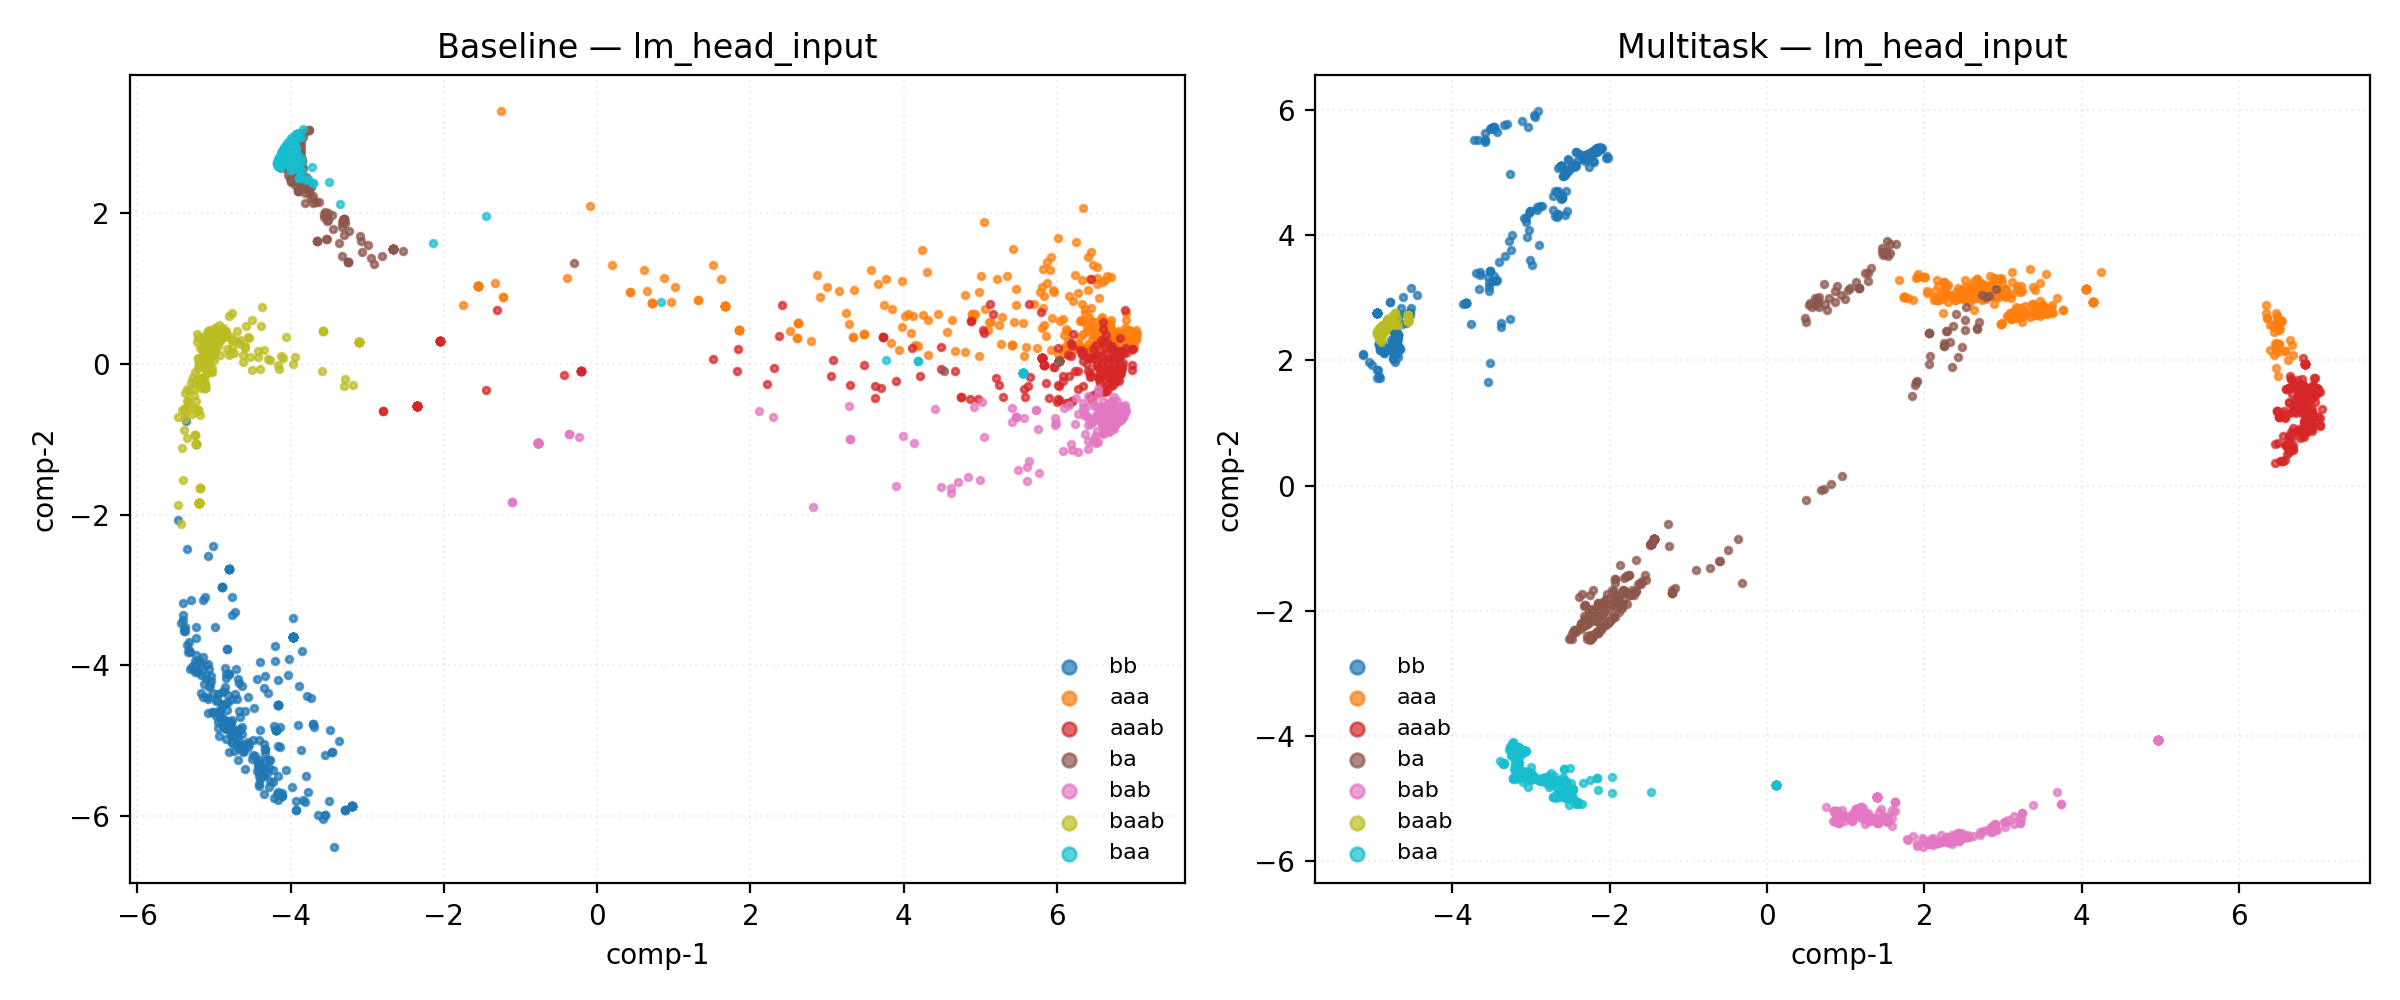
\includegraphics[width=0.9\textwidth]{../../../entanglement_plots/latent_space_eps_dist_vs_baseline.png}
\caption{PCA visualization showing dramatic improvement in latent space organization with multitask learning (left: baseline, right: multitask)}
\label{fig:multitask-pca}
\end{figure}

\section{Out-of-Distribution Robustness}
\label{sec:ood}

\subsection{OOD Evaluation Framework}

We test model robustness under six distribution shift scenarios:

\begin{table}[htbp]
\centering
\caption{OOD test regimes and their characteristics}
\label{tab:ood-regimes}
\begin{tabular}{@{}lp{8cm}@{}}
\toprule
\textbf{Regime} & \textbf{Description} \\
\midrule
Emission mix & Interpolate emissions toward uniform distribution \\
Start state uniform & Randomize initial state distribution \\
Transition noise & Add random state jumps with probability $p$ \\
Alphabet swap & Globally permute 0↔1 mapping \\
State-dependent swap & Swap emissions for subset of states \\
Temporal swap & Time-varying emission permutation \\
\bottomrule
\end{tabular}
\end{table}

\subsection{Adaptation Strategies}

\begin{keyresult}[OOD Adaptation Results]
Multitask models show superior adaptability:

\begin{itemize}
    \item \textbf{Zero-shot}: Multitask maintains better structure under shifts
    \item \textbf{Head remapping}: Simple 2×2 matrix recovers performance
    \item \textbf{Few-shot}: 16 context tokens enable effective adaptation
    \item \textbf{State-aware}: Per-state calibration handles complex shifts
\end{itemize}
\end{keyresult}

\begin{table}[htbp]
\centering
\caption{OOD performance comparison (alphabet swap regime)}
\label{tab:ood-alphabet}
\begin{tabular}{@{}lccc@{}}
\toprule
\textbf{Setting} & \textbf{Baseline} & \textbf{$\epsmachine$-head} & \textbf{$\epsmachine$+dist} \\
\midrule
Raw (zero-shot) & 2.656 & 2.735 & 2.817 \\
Calibrated & 0.539 & 0.527 & \cellcolor{highlightgreen}0.523 \\
Few-shot (16 tokens) & 0.548 & 0.535 & \cellcolor{highlightgreen}0.531 \\
\bottomrule
\end{tabular}
\end{table}

\chapter{Conclusions and Future Directions}
\label{ch:conclusions}

\section{Summary of Contributions}
\label{sec:summary}

This work presents Neural CSSR, a robust solution to epsilon machine discovery that overcomes fundamental limitations of classical approaches:

\begin{enumerate}
    \item \textbf{Theoretical contribution}: Established the connection between neural sequence models and computational mechanics, proving that transformer predictions can recover causal state structure.
    
    \item \textbf{Algorithmic innovation}: Developed a three-stage discovery algorithm using JS divergence clustering that eliminates parameter brittleness and handles infinite memory processes.
    
    \item \textbf{Empirical validation}: Demonstrated perfect state recovery on challenging benchmarks where classical methods fail, including the Seven-State Human and infinite-memory Even Process.
    
    \item \textbf{Representation insights}: Showed why output-based discovery succeeds despite entangled hidden representations, validating the functional approach to causal state identification.
    
    \item \textbf{Practical extensions}: Explored multitask learning for improved representations and OOD robustness through adaptive calibration.
\end{enumerate}

\section{Implications for Computational Mechanics}
\label{sec:implications}

Neural CSSR bridges two traditionally separate fields:

\begin{notebox}[Bridging Deep Learning and Computational Mechanics]
\begin{itemize}
    \item \textbf{For computational mechanics}: Neural networks provide robust probability estimation that overcomes sampling limitations
    \item \textbf{For deep learning}: Epsilon machines offer interpretable structure discovery for sequence models
    \item \textbf{For applications}: Practical epsilon machine discovery becomes feasible for real-world data
\end{itemize}
\end{notebox}

\section{Future Research Directions}
\label{sec:future}

\subsection{Methodological Extensions}

\begin{enumerate}
    \item \textbf{Continuous state spaces}: Extend to processes with continuous observations
    \item \textbf{Non-stationary processes}: Handle time-varying causal structure
    \item \textbf{Hierarchical discovery}: Learn multi-scale epsilon machines
    \item \textbf{Online adaptation}: Develop streaming algorithms for evolving processes
\end{enumerate}

\subsection{Applications}

\begin{enumerate}
    \item \textbf{Neuroscience}: Analyze neural spike trains and brain state dynamics
    \item \textbf{Finance}: Model market microstructure and regime changes
    \item \textbf{Climate}: Discover causal patterns in climate time series
    \item \textbf{Biology}: Understand gene regulatory dynamics
\end{enumerate}

\subsection{Theoretical Questions}

\begin{enumerate}
    \item What is the sample complexity of neural epsilon machine discovery?
    \item Can we prove convergence guarantees for the three-stage algorithm?
    \item How do architectural choices affect discovered causal structure?
    \item What is the relationship between transformer attention and causal states?
\end{enumerate}

\section{Closing Remarks}
\label{sec:closing}

Neural CSSR represents a significant advance in automated causal structure discovery, making epsilon machine reconstruction practical for complex real-world processes. By combining the representational power of neural networks with the theoretical rigor of computational mechanics, we open new possibilities for understanding and modeling sequential phenomena across scientific disciplines.

The success of our approach—achieving perfect state recovery where classical methods fail—demonstrates that neural networks can serve not just as black-box predictors but as tools for discovering interpretable causal structure. This work is a step toward the broader goal of extracting meaningful, minimal representations from complex sequential data.

% Appendices
\appendix

\chapter{Algorithm Pseudocode}
\label{app:algorithms}

\section{Complete Three-Stage Algorithm}

\begin{algorithm}[htbp]
\caption{Complete Neural CSSR Algorithm}
\label{alg:complete-neural-cssr}
\SetAlgoLined
\KwIn{Model checkpoint, data, parameters $\tau_A$, $\tau_B$, $L$, $k$}
\KwOut{Epsilon machine $\epsmachine$}

\tcp{Phase 1: Sample and compute emissions}
$\histories \leftarrow$ SampleHistories(data, $n$, $L$) \;
\ForEach{$h \in \histories$}{
    $P_h \leftarrow$ NeuralPredict(model, $h$) \;
}

\tcp{Phase 2: Three-stage clustering}
\tcp{Stage A: Emission clustering}
$\mathcal{C}_A \leftarrow$ AgglomerativeCluster($\histories$, $P$, $\tau_A$) \;

\tcp{Stage A+: Backward stability (optional)}
\If{backward\_stability\_enabled}{
    \ForEach{cluster $c \in \mathcal{C}_A$}{
        $\mathcal{C}_A' \leftarrow$ BackwardStabilityRefine($c$, tolerance) \;
    }
}

\tcp{Stage B: Conditional refinement}
$\mathcal{C}_B \leftarrow \emptyset$ \;
\ForEach{group $g \in \mathcal{C}_A$}{
    representatives $\leftarrow$ SelectRepresentatives($g$) \;
    refined $\leftarrow$ ConditionalJSCluster(representatives, $\tau_B$, $k$) \;
    $\mathcal{C}_B \leftarrow \mathcal{C}_B \cup$ refined \;
}

\tcp{Stage C: State remerging (optional)}
\If{remerging\_enabled}{
    $\mathcal{C}_C \leftarrow$ FunctionalMerge($\mathcal{C}_B$, $\epsilon_{\text{emit}}$, $\epsilon_{\text{rollout}}$) \;
}
\Else{
    $\mathcal{C}_C \leftarrow \mathcal{C}_B$ \;
}

\tcp{Phase 3: Build epsilon machine}
$\states \leftarrow$ ExtractStates($\mathcal{C}_C$) \;
$T \leftarrow$ LearnTransitions($\states$, data) \;
$\epsilon \leftarrow$ LearnEmissions($\states$) \;

\Return{$(\states, T, \epsilon)$}
\end{algorithm}

\chapter{Extended Experimental Data}
\label{app:experimental}

\section{Detailed Seven-State Results}

\begin{table}[htbp]
\centering
\caption{Complete clustering progression for Seven-State Human}
\label{tab:seven-state-detailed}
\small
\begin{tabular}{@{}lccccl@{}}
\toprule
\textbf{Stage} & \textbf{Iteration} & \textbf{Clusters} & \textbf{Min JS} & \textbf{Max JS} & \textbf{Action} \\
\midrule
\multirow{5}{*}{Stage A} 
& 0 & 30 & -- & -- & Initialize \\
& 5 & 25 & 0.0001 & 0.0008 & Merging \\
& 10 & 20 & 0.0003 & 0.0015 & Merging \\
& 20 & 10 & 0.0008 & 0.0045 & Merging \\
& 26 & 5 & 0.0012 & 0.0089 & Stop \\
\midrule
\multirow{3}{*}{Backward} 
& -- & 5 groups & -- & -- & Input \\
& -- & 7 contexts & -- & -- & Refined \\
& -- & -- & -- & -- & 70 tokens dropped \\
\midrule
Stage B & -- & 7 & 0.0021 & 0.0156 & No merges \\
\bottomrule
\end{tabular}
\end{table}

\section{Parameter Sensitivity Analysis}

\begin{table}[htbp]
\centering
\caption{Parameter sensitivity for different thresholds}
\label{tab:parameter-sensitivity}
\begin{tabular}{@{}cccccc@{}}
\toprule
\textbf{Process} & \textbf{$\tau_A$} & \textbf{$\tau_B$} & \textbf{States} & \textbf{Purity} & \textbf{Loss} \\
\midrule
\multirow{4}{*}{Seven-State}
& 0.0001 & 0.001 & 9 & 95\% & 0.78 \\
& 0.0005 & 0.001 & 7 & 98\% & 0.77 \\
& \cellcolor{highlightgreen}0.001 & \cellcolor{highlightgreen}0.001 & \cellcolor{highlightgreen}7 & \cellcolor{highlightgreen}100\% & \cellcolor{highlightgreen}0.77 \\
& 0.005 & 0.001 & 5 & 88\% & 0.81 \\
\midrule
\multirow{4}{*}{Even Process}
& 0.0001 & 0.001 & 8 & 92\% & 0.85 \\
& 0.0005 & 0.001 & 5 & 96\% & 0.82 \\
& \cellcolor{highlightgreen}0.001 & \cellcolor{highlightgreen}0.001 & \cellcolor{highlightgreen}3 & \cellcolor{highlightgreen}100\% & \cellcolor{highlightgreen}0.80 \\
& 0.005 & 0.001 & 2 & 94\% & 0.88 \\
\bottomrule
\end{tabular}
\end{table}

\chapter{Mathematical Proofs}
\label{app:proofs}

\section{JS Divergence Properties}

\begin{proof}[Proof of JS metric property]
We prove that $\sqrt{\JS(P,Q)}$ satisfies the metric axioms.

\textbf{Non-negativity and identity}: 
$\JS(P,Q) \geq 0$ with equality iff $P = Q$ follows from KL divergence properties.

\textbf{Symmetry}: 
By construction, $\JS(P,Q) = \frac{1}{2}[\KL(P||M) + \KL(Q||M)]$ where $M = \frac{P+Q}{2}$.
Since the roles of $P$ and $Q$ are symmetric, $\JS(P,Q) = \JS(Q,P)$.

\textbf{Triangle inequality}: 
For the square root, we need to show:
$$\sqrt{\JS(P,R)} \leq \sqrt{\JS(P,Q)} + \sqrt{\JS(Q,R)}$$

This follows from the fact that $\sqrt{\JS}$ can be expressed as the $L^2$ distance between square-root probability vectors after an appropriate transformation, inheriting the triangle inequality from Euclidean space.
\end{proof}

\section{Convergence of Three-Stage Algorithm}

\begin{theorem}[Convergence of Stage A]
\label{thm:stage-a-convergence}
Stage A agglomerative clustering with threshold $\tau_A$ converges to a unique partition in $O(n^2 \log n)$ time, where $n$ is the number of initial histories.
\end{theorem}

\begin{proof}[Proof sketch]
The algorithm maintains a priority queue of pairwise JS divergences. At each step:
\begin{enumerate}
    \item The minimum divergence pair is selected: $O(\log n)$
    \item The pair is merged if below threshold
    \item Divergences to the new cluster are recomputed: $O(n)$
    \item The process continues until no pairs below threshold exist
\end{enumerate}

Since we perform at most $n-1$ merges and each requires $O(n)$ divergence computations, the total complexity is $O(n^2 \log n)$.

Uniqueness follows from the deterministic greedy selection of minimum divergence pairs and the strict ordering imposed by the JS metric.
\end{proof}

% Bibliography (placeholder - would use BibTeX in production)
\chapter*{References}
\addcontentsline{toc}{chapter}{References}

\begin{enumerate}
\item Crutchfield, J. P., \& Young, K. (1989). Inferring statistical complexity. \textit{Physical Review Letters}, 63(2), 105.

\item Shalizi, C. R., \& Crutchfield, J. P. (2001). Computational mechanics: Pattern and prediction, structure and simplicity. \textit{Journal of Statistical Physics}, 104(3-4), 817-879.

\item Vaswani, A., et al. (2017). Attention is all you need. \textit{Advances in Neural Information Processing Systems}, 30.

\item Lin, J. (1991). Divergence measures based on the Shannon entropy. \textit{IEEE Transactions on Information Theory}, 37(1), 145-151.

\item Platt, J. (1999). Probabilistic outputs for support vector machines and comparisons to regularized likelihood methods. \textit{Advances in Large Margin Classifiers}, 10(3), 61-74.
\end{enumerate}

% Index placeholder
\chapter*{Index}
\addcontentsline{toc}{chapter}{Index}

\noindent
Agglomerative clustering, 25, 31 \\
Backward stability, 28, 35, 42 \\
Calibration, 30, 58 \\
Causal equivalence, 15, 22 \\
Conditional JS divergence, 29, 36 \\
Entropy rate, 16, 45 \\
Epsilon machine, 13, 15, 22 \\
Even Process, 19, 44-48 \\
Golden Mean, 18, 40 \\
Hidden representations, 52-54 \\
Jensen-Shannon divergence, 24, 50-51 \\
Multitask learning, 55-57 \\
Neural CSSR, 21-38 \\
Out-of-distribution, 58-60 \\
Platt scaling, 30 \\
Seven-State Human, 19, 41-43 \\
Stage A/B/C, 26-29 \\
Statistical complexity, 16 \\
Three-stage algorithm, 25-29 \\
Transformer architecture, 30 \\

\end{document}
